%! Author = hxp
%! Date = 2020-11-09

\documentclass{ctexart}


\usepackage{ctex}
\usepackage{amsmath}
\usepackage{amsfonts}
\usepackage{amssymb}
\usepackage{wasysym}
\newcommand{\angstrom}{\text{\normalfont\AA}}  % 定义了原子物理的A
\usepackage{graphicx}
\usepackage{float}
\restylefloat{table}
\usepackage{geometry}
\geometry{a4paper,scale=0.8}  % 定义页面大小是A4,缩放是0.8
\usepackage{caption}
\usepackage{subcaption}
\usepackage{enumitem}

\newcommand*{\md}{\mathop{}\!\mathrm{d}}   % 定义微分算子,直立体的d
\newcommand*{\me}{\mathrm{e}}              % 定义自然对数e,同样应当是直立体

% 如果你想要每一段的开头不要空两格,注释掉下面这两行
\usepackage{parskip}
\setlength{\parindent}{0cm}

% 默认的\mathbf对希腊字母不生效,这里改下
\usepackage{bm}
\let\Oldmathbf\mathbf
\renewcommand{\mathbf}[1]{\boldsymbol{\Oldmathbf{#1}}}

% 表格默认格内内容和边框没有留出距离,显示分数的时候,分数的上下会贴到边框上
% 因此我增加了表格内容和边框的最短距离是5像素
\usepackage{cellspace}
\setlength{\cellspacetoplimit}{5pt}
\setlength{\cellspacebottomlimit}{5pt}

% \si命令是用来写单位的,单位需要和之前的数字有一个空格的距离,而且应当直立体
% 用法:5 \si{km/h}
\newcommand{\si}[1]{\  \mathrm{#1}}

% 日期不要显示
\date{}

\usepackage{fancyhdr}
\pagestyle{fancy}
\fancyhf{}
\lhead{本文档TeX源码地址:https://github.com/hxp-plus/Notes/tree/master/Physics-Experiment/实验报告}
\rfoot{第 \thepage 页}
\renewcommand{\headrulewidth}{1pt}
\renewcommand{\footrulewidth}{1pt}

%% 标题三号黑体,作者信息为班级姓名学号
\newcommand{\generatetitle}[6]{\title{\zihao{3}\heiti#1} \author{#2 \quad
\quad #3 \quad\quad #4 \quad\quad #5 \quad\quad #6} \maketitle\thispagestyle{fancy}}

%% 所有的引言、实验内容与数据处理啥的,用section
\ctexset {
section = {
format = \raggedright\zihao{4}\heiti,  % 设置所有section的字号为四号黑体左对齐
name={,、},                            % 序号后跟顿号
aftername={\hspace{0pt}},              % 修改序号和标题直接的间距为零
number=\chinese{section},              % 设置序号为中文
},
subsection = {
format = \raggedright\zihao{5}\heiti,  % 设置所有subsection的字号为五号黑体左对齐
number={},              % 设置序号为没有序号
},
subsubsection = {
format = \raggedright\zihao{5}\heiti,  % 设置所有subsection的字号为五号黑体左对齐
number={},              % 设置序号为没有序号
}
}

%% 实验背景、实验目的啥的,用subsection
\ctexset {
subsection = {
format = \raggedright\zihao{5}\heiti,  % 所有subsection的字号为五号黑体左对齐
number={},                             % 设置序号为没有序号
}
}

%% 把subsection之间加上中括号
\let\oldsubsection\subsection
\renewcommand{\subsection}[1]{\oldsubsection{\!\!\!\!\!\!【#1】}}
\let\oldsubsubsection\subsubsection
\renewcommand{\subsubsection}[1]{\oldsubsubsection{\!\!\!\!\!\!【#1】}}

%% 摘要和关键词用paragraph

\ctexset {
paragraph = {
format = \raggedright\zihao{5}\heiti,  % 所有paragraph的字号为五号黑体左对齐
number={},                             % 设置序号为没有序号
}
}

%% 把paragraph之间加上中括号
\let\oldparagraph\paragraph
\renewcommand{\paragraph}[1]{\oldparagraph{#1:\!\!\!\!\!\!}}

%% 再把参考文献的序号去掉
\makeatletter
\renewcommand\@biblabel[1]{}
\makeatother

\begin{document}

    \generatetitle{综合物理实验报告——
    综合光学实验}{物理4+4}{胡喜平}{U201811966}{hxp@hust.edu.cn}{https://hxp.plus/}

    \paragraph{摘要}

    \paragraph{关键词}


    \section{引言}

    \subsection{实验目的}


    \section{实验内容与数据处理}

    \subsection{实验原理}

    \subsection{实验内容}

    \subsection{实验结果的分析和结论}

    \newpage
    \begin{table}[H]
        \centering
        \begin{tabular}{|c|c|c|c|c|c|c|c|c|}
            \hline
            励磁电流($\si{A}$)   & 0    & 0.3  & 0.6  & 0.9  & 1.2  & 1.5  & 1.8  & 2.0  \\\hline
            磁场强度($\si{mT}$)  & 0.00 & 0.00 & 0.00 & 0.00 & 0.00 & 0.00 & 0.00 & 0.00 \\\hline
            反向励磁电流($\si{A}$) & 0    & 0.3  & 0.6  & 0.9  & 1.2  & 1.5  & 1.8  & 2.0  \\\hline
            磁场强度($\si{mT}$)  & 0.00 & 0.00 & 0.00 & 0.00 & 0.00 & 0.00 & 0.00 & 0.00 \\\hline
        \end{tabular}
        \caption{励磁电流和磁场强度关系}
    \end{table}
    \newpage
    \begin{table}[H]
        \centering
        \begin{tabular}{|c|c|c|c|c|c|c|c|c|c|}
            \hline
            检偏镜角度(${}^{\circ}$)  & 0    & 10   & 20   & 30   & 40   & 50   & 60   & 70   & 80   \\\hline
            光强($10^{-7} \si{A}$) & 0.00 & 0.00 & 0.00 & 0.00 & 0.00 & 0.00 & 0.00 & 0.00 & 0.00 \\\hline
            检偏镜角度(${}^{\circ}$)  & 90   & 100  & 110  & 120  & 130  & 140  & 150  & 160  & 170  \\\hline
            光强($10^{-7} \si{A}$) & 0.00 & 0.00 & 0.00 & 0.00 & 0.00 & 0.00 & 0.00 & 0.00 & 0.00 \\\hline
            检偏镜角度(${}^{\circ}$)  & 180  & 190  & 200  & 210  & 220  & 230  & 240  & 250  & 260  \\\hline
            光强($10^{-7} \si{A}$) & 0.00 & 0.00 & 0.00 & 0.00 & 0.00 & 0.00 & 0.00 & 0.00 & 0.00 \\\hline
            检偏镜角度(${}^{\circ}$)  & 270  & 280  & 290  & 300  & 310  & 320  & 330  & 340  & 350  \\\hline
            光强($10^{-7} \si{A}$) & 0.00 & 0.00 & 0.00 & 0.00 & 0.00 & 0.00 & 0.00 & 0.00 & 0.00 \\\hline
        \end{tabular}
        \caption{检偏器角度与光强关系,特定励磁电流$I=0.00 \si{A}$}
    \end{table}

    \begin{figure}[H]
        \centering
        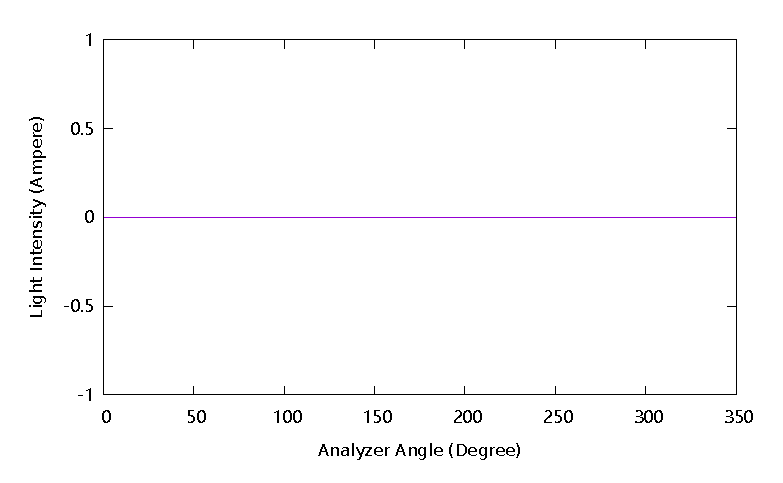
\includegraphics[width=\linewidth]{../output/analyzer-angle-light-intensity-1.gnuplot}
    \end{figure}
    \newpage
    \begin{table}[H]
        \centering
        \begin{tabular}{|c|c|c|c|c|c|c|c|c|c|}
            \hline
            检偏镜角度(${}^{\circ}$)  & 0    & 10   & 20   & 30   & 40   & 50   & 60   & 70   & 80   \\\hline
            光强($10^{-7} \si{A}$) & 0.00 & 0.00 & 0.00 & 0.00 & 0.00 & 0.00 & 0.00 & 0.00 & 0.00 \\\hline
            检偏镜角度(${}^{\circ}$)  & 90   & 100  & 110  & 120  & 130  & 140  & 150  & 160  & 170  \\\hline
            光强($10^{-7} \si{A}$) & 0.00 & 0.00 & 0.00 & 0.00 & 0.00 & 0.00 & 0.00 & 0.00 & 0.00 \\\hline
            检偏镜角度(${}^{\circ}$)  & 180  & 190  & 200  & 210  & 220  & 230  & 240  & 250  & 260  \\\hline
            光强($10^{-7} \si{A}$) & 0.00 & 0.00 & 0.00 & 0.00 & 0.00 & 0.00 & 0.00 & 0.00 & 0.00 \\\hline
            检偏镜角度(${}^{\circ}$)  & 270  & 280  & 290  & 300  & 310  & 320  & 330  & 340  & 350  \\\hline
            光强($10^{-7} \si{A}$) & 0.00 & 0.00 & 0.00 & 0.00 & 0.00 & 0.00 & 0.00 & 0.00 & 0.00 \\\hline
        \end{tabular}
        \caption{检偏器角度与光强关系,特定励磁电流$I=0.00 \si{A}$}
    \end{table}

    \begin{figure}[H]
        \centering
        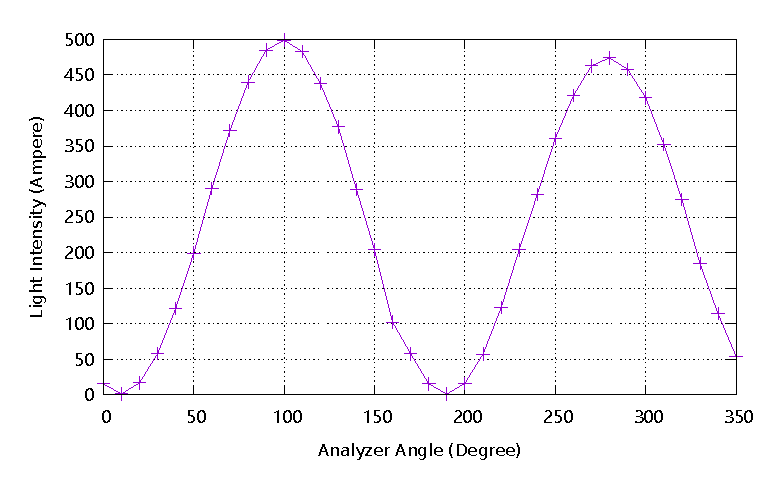
\includegraphics[width=\linewidth]{../output/analyzer-angle-light-intensity-2.gnuplot}
    \end{figure}
    \newpage
    \begin{table}[H]
        \centering
        \begin{tabular}{|c|c|c|c|c|c|c|c|c|c|}
            \hline
            检偏镜角度(${}^{\circ}$)  & 0    & 10   & 20   & 30   & 40   & 50   & 60   & 70   & 80   \\\hline
            光强($10^{-7} \si{A}$) & 0.00 & 0.00 & 0.00 & 0.00 & 0.00 & 0.00 & 0.00 & 0.00 & 0.00 \\\hline
            检偏镜角度(${}^{\circ}$)  & 90   & 100  & 110  & 120  & 130  & 140  & 150  & 160  & 170  \\\hline
            光强($10^{-7} \si{A}$) & 0.00 & 0.00 & 0.00 & 0.00 & 0.00 & 0.00 & 0.00 & 0.00 & 0.00 \\\hline
            检偏镜角度(${}^{\circ}$)  & 180  & 190  & 200  & 210  & 220  & 230  & 240  & 250  & 260  \\\hline
            光强($10^{-7} \si{A}$) & 0.00 & 0.00 & 0.00 & 0.00 & 0.00 & 0.00 & 0.00 & 0.00 & 0.00 \\\hline
            检偏镜角度(${}^{\circ}$)  & 270  & 280  & 290  & 300  & 310  & 320  & 330  & 340  & 350  \\\hline
            光强($10^{-7} \si{A}$) & 0.00 & 0.00 & 0.00 & 0.00 & 0.00 & 0.00 & 0.00 & 0.00 & 0.00 \\\hline
        \end{tabular}
        \caption{检偏器角度与光强关系,特定励磁电流$I=0.00 \si{A}$}
    \end{table}

    \begin{figure}[H]
        \centering
        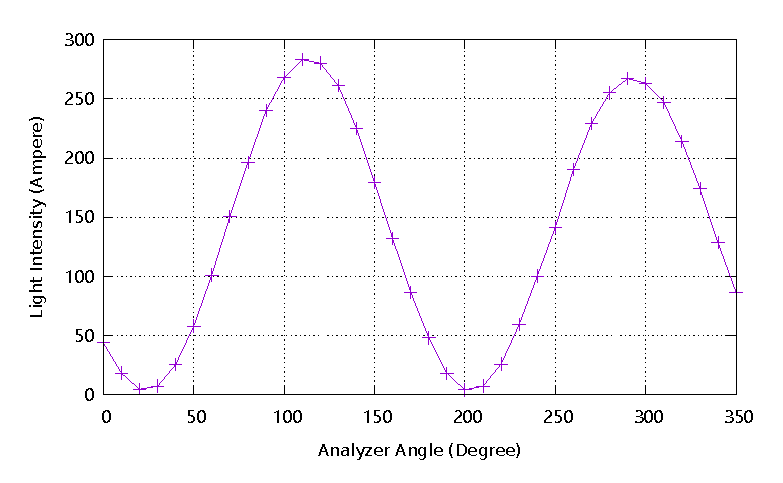
\includegraphics[width=\linewidth]{../output/analyzer-angle-light-intensity-3.gnuplot}
    \end{figure}
    \newpage
    \begin{table}[H]
        \centering
        \begin{tabular}{|c|c|c|c|c|c|c|c|c|c|}
            \hline
            检偏镜角度(${}^{\circ}$)  & 0    & 10   & 20   & 30   & 40   & 50   & 60   & 70   & 80   \\\hline
            光强($10^{-7} \si{A}$) & 0.00 & 0.00 & 0.00 & 0.00 & 0.00 & 0.00 & 0.00 & 0.00 & 0.00 \\\hline
            检偏镜角度(${}^{\circ}$)  & 90   & 100  & 110  & 120  & 130  & 140  & 150  & 160  & 170  \\\hline
            光强($10^{-7} \si{A}$) & 0.00 & 0.00 & 0.00 & 0.00 & 0.00 & 0.00 & 0.00 & 0.00 & 0.00 \\\hline
            检偏镜角度(${}^{\circ}$)  & 180  & 190  & 200  & 210  & 220  & 230  & 240  & 250  & 260  \\\hline
            光强($10^{-7} \si{A}$) & 0.00 & 0.00 & 0.00 & 0.00 & 0.00 & 0.00 & 0.00 & 0.00 & 0.00 \\\hline
            检偏镜角度(${}^{\circ}$)  & 270  & 280  & 290  & 300  & 310  & 320  & 330  & 340  & 350  \\\hline
            光强($10^{-7} \si{A}$) & 0.00 & 0.00 & 0.00 & 0.00 & 0.00 & 0.00 & 0.00 & 0.00 & 0.00 \\\hline
        \end{tabular}
        \caption{检偏器角度与光强关系,特定励磁电流$I=0.00 \si{A}$}
    \end{table}

    \begin{figure}[H]
        \centering
        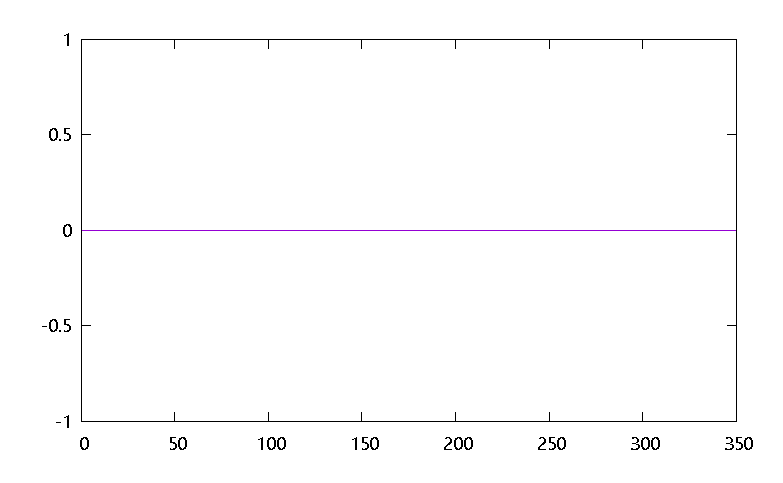
\includegraphics[width=\linewidth]{../output/analyzer-angle-light-intensity-4.gnuplot}
    \end{figure}
    \newpage
    \begin{table}[H]
        \centering
        \begin{tabular}{|c|c|c|c|c|c|c|c|c|c|}
            \hline
            检偏镜角度(${}^{\circ}$)  & 0    & 10   & 20   & 30   & 40   & 50   & 60   & 70   & 80   \\\hline
            光强($10^{-7} \si{A}$) & 0.00 & 0.00 & 0.00 & 0.00 & 0.00 & 0.00 & 0.00 & 0.00 & 0.00 \\\hline
            检偏镜角度(${}^{\circ}$)  & 90   & 100  & 110  & 120  & 130  & 140  & 150  & 160  & 170  \\\hline
            光强($10^{-7} \si{A}$) & 0.00 & 0.00 & 0.00 & 0.00 & 0.00 & 0.00 & 0.00 & 0.00 & 0.00 \\\hline
            检偏镜角度(${}^{\circ}$)  & 180  & 190  & 200  & 210  & 220  & 230  & 240  & 250  & 260  \\\hline
            光强($10^{-7} \si{A}$) & 0.00 & 0.00 & 0.00 & 0.00 & 0.00 & 0.00 & 0.00 & 0.00 & 0.00 \\\hline
            检偏镜角度(${}^{\circ}$)  & 270  & 280  & 290  & 300  & 310  & 320  & 330  & 340  & 350  \\\hline
            光强($10^{-7} \si{A}$) & 0.00 & 0.00 & 0.00 & 0.00 & 0.00 & 0.00 & 0.00 & 0.00 & 0.00 \\\hline
        \end{tabular}
        \caption{检偏器角度与光强关系,特定励磁电流$I=0.00 \si{A}$}
    \end{table}

    \begin{figure}[H]
        \centering
        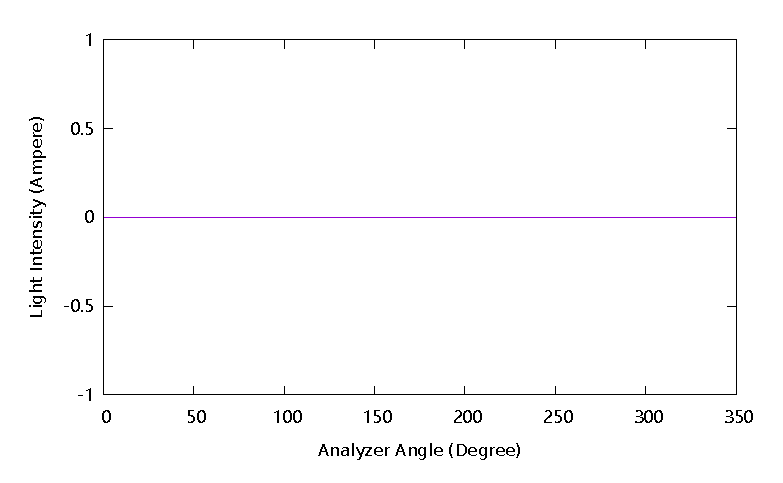
\includegraphics[width=\linewidth]{../output/analyzer-angle-light-intensity-5.gnuplot}
    \end{figure}
    \newpage
    \begin{table}[H]
        \centering
        \begin{tabular}{|c|c|c|c|c|c|c|c|c|c|}
            \hline
            检偏镜角度(${}^{\circ}$)  & 0    & 10   & 20   & 30   & 40   & 50   & 60   & 70   & 80   \\\hline
            光强($10^{-7} \si{A}$) & 0.00 & 0.00 & 0.00 & 0.00 & 0.00 & 0.00 & 0.00 & 0.00 & 0.00 \\\hline
            检偏镜角度(${}^{\circ}$)  & 90   & 100  & 110  & 120  & 130  & 140  & 150  & 160  & 170  \\\hline
            光强($10^{-7} \si{A}$) & 0.00 & 0.00 & 0.00 & 0.00 & 0.00 & 0.00 & 0.00 & 0.00 & 0.00 \\\hline
            检偏镜角度(${}^{\circ}$)  & 180  & 190  & 200  & 210  & 220  & 230  & 240  & 250  & 260  \\\hline
            光强($10^{-7} \si{A}$) & 0.00 & 0.00 & 0.00 & 0.00 & 0.00 & 0.00 & 0.00 & 0.00 & 0.00 \\\hline
            检偏镜角度(${}^{\circ}$)  & 270  & 280  & 290  & 300  & 310  & 320  & 330  & 340  & 350  \\\hline
            光强($10^{-7} \si{A}$) & 0.00 & 0.00 & 0.00 & 0.00 & 0.00 & 0.00 & 0.00 & 0.00 & 0.00 \\\hline
        \end{tabular}
        \caption{检偏器角度与光强关系,特定励磁电流$I=0.00 \si{A}$}
    \end{table}

    \begin{figure}[H]
        \centering
        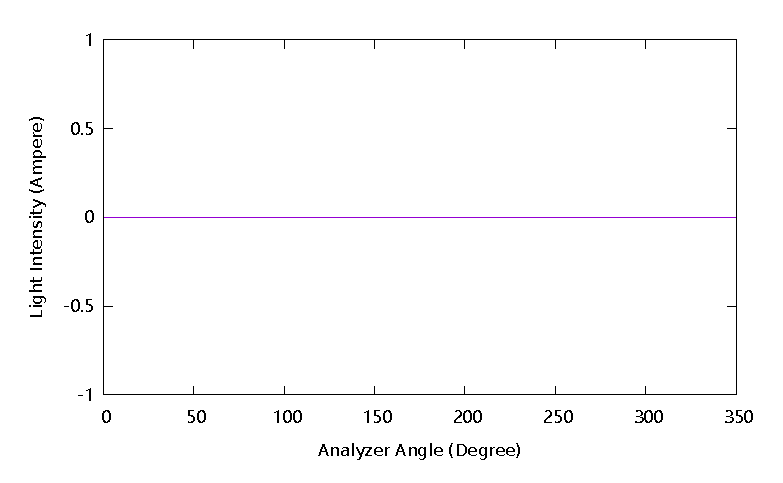
\includegraphics[width=\linewidth]{../output/analyzer-angle-light-intensity-6.gnuplot}
    \end{figure}
    \newpage
    \begin{table}[H]
        \centering
        \begin{tabular}{|c|c|c|c|c|c|c|c|c|c|}
            \hline
            检偏镜角度(${}^{\circ}$)  & 0    & 10   & 20   & 30   & 40   & 50   & 60   & 70   & 80   \\\hline
            光强($10^{-7} \si{A}$) & 0.00 & 0.00 & 0.00 & 0.00 & 0.00 & 0.00 & 0.00 & 0.00 & 0.00 \\\hline
            检偏镜角度(${}^{\circ}$)  & 90   & 100  & 110  & 120  & 130  & 140  & 150  & 160  & 170  \\\hline
            光强($10^{-7} \si{A}$) & 0.00 & 0.00 & 0.00 & 0.00 & 0.00 & 0.00 & 0.00 & 0.00 & 0.00 \\\hline
            检偏镜角度(${}^{\circ}$)  & 180  & 190  & 200  & 210  & 220  & 230  & 240  & 250  & 260  \\\hline
            光强($10^{-7} \si{A}$) & 0.00 & 0.00 & 0.00 & 0.00 & 0.00 & 0.00 & 0.00 & 0.00 & 0.00 \\\hline
            检偏镜角度(${}^{\circ}$)  & 270  & 280  & 290  & 300  & 310  & 320  & 330  & 340  & 350  \\\hline
            光强($10^{-7} \si{A}$) & 0.00 & 0.00 & 0.00 & 0.00 & 0.00 & 0.00 & 0.00 & 0.00 & 0.00 \\\hline
        \end{tabular}
        \caption{检偏器角度与光强关系,特定励磁电流$I=0.00 \si{A}$}
    \end{table}

    \begin{figure}[H]
        \centering
        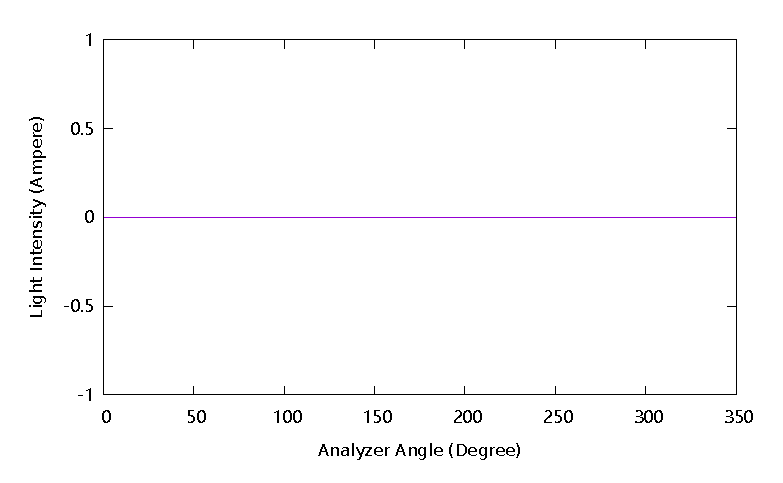
\includegraphics[width=\linewidth]{../output/analyzer-angle-light-intensity-7.gnuplot}
    \end{figure}
    \newpage
    \begin{table}[H]
        \centering
        \begin{tabular}{|c|c|c|c|c|c|c|c|c|c|}
            \hline
            检偏镜角度(${}^{\circ}$)  & 0    & 10   & 20   & 30   & 40   & 50   & 60   & 70   & 80   \\\hline
            光强($10^{-7} \si{A}$) & 0.00 & 0.00 & 0.00 & 0.00 & 0.00 & 0.00 & 0.00 & 0.00 & 0.00 \\\hline
            检偏镜角度(${}^{\circ}$)  & 90   & 100  & 110  & 120  & 130  & 140  & 150  & 160  & 170  \\\hline
            光强($10^{-7} \si{A}$) & 0.00 & 0.00 & 0.00 & 0.00 & 0.00 & 0.00 & 0.00 & 0.00 & 0.00 \\\hline
            检偏镜角度(${}^{\circ}$)  & 180  & 190  & 200  & 210  & 220  & 230  & 240  & 250  & 260  \\\hline
            光强($10^{-7} \si{A}$) & 0.00 & 0.00 & 0.00 & 0.00 & 0.00 & 0.00 & 0.00 & 0.00 & 0.00 \\\hline
            检偏镜角度(${}^{\circ}$)  & 270  & 280  & 290  & 300  & 310  & 320  & 330  & 340  & 350  \\\hline
            光强($10^{-7} \si{A}$) & 0.00 & 0.00 & 0.00 & 0.00 & 0.00 & 0.00 & 0.00 & 0.00 & 0.00 \\\hline
        \end{tabular}
        \caption{检偏器角度与光强关系,特定励磁电流$I=0.00 \si{A}$}
    \end{table}

    \begin{figure}[H]
        \centering
        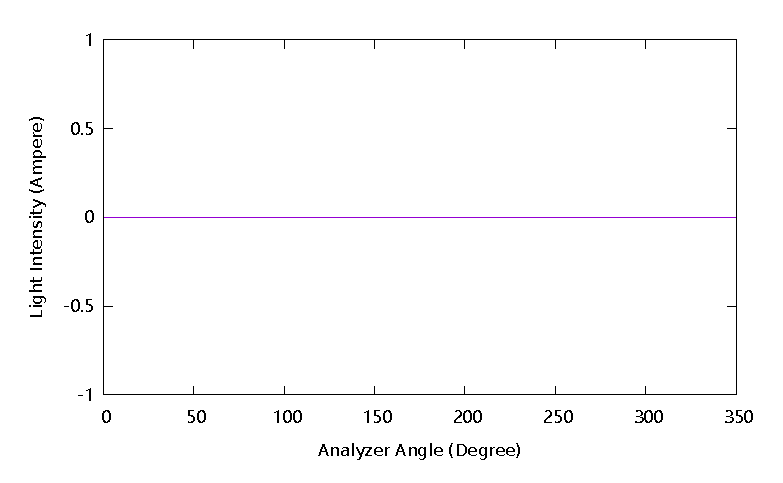
\includegraphics[width=\linewidth]{../output/analyzer-angle-light-intensity-8.gnuplot}
    \end{figure}
    \newpage
    \begin{table}[H]
        \centering
        \begin{tabular}{|c|c|c|c|c|c|c|c|c|c|}
            \hline
            检偏镜角度(${}^{\circ}$)  & 0    & 10   & 20   & 30   & 40   & 50   & 60   & 70   & 80   \\\hline
            光强($10^{-7} \si{A}$) & 0.00 & 0.00 & 0.00 & 0.00 & 0.00 & 0.00 & 0.00 & 0.00 & 0.00 \\\hline
            检偏镜角度(${}^{\circ}$)  & 90   & 100  & 110  & 120  & 130  & 140  & 150  & 160  & 170  \\\hline
            光强($10^{-7} \si{A}$) & 0.00 & 0.00 & 0.00 & 0.00 & 0.00 & 0.00 & 0.00 & 0.00 & 0.00 \\\hline
            检偏镜角度(${}^{\circ}$)  & 180  & 190  & 200  & 210  & 220  & 230  & 240  & 250  & 260  \\\hline
            光强($10^{-7} \si{A}$) & 0.00 & 0.00 & 0.00 & 0.00 & 0.00 & 0.00 & 0.00 & 0.00 & 0.00 \\\hline
            检偏镜角度(${}^{\circ}$)  & 270  & 280  & 290  & 300  & 310  & 320  & 330  & 340  & 350  \\\hline
            光强($10^{-7} \si{A}$) & 0.00 & 0.00 & 0.00 & 0.00 & 0.00 & 0.00 & 0.00 & 0.00 & 0.00 \\\hline
        \end{tabular}
        \caption{检偏器角度与光强关系,特定励磁电流$I=0.00 \si{A}$}
    \end{table}

    \begin{figure}[H]
        \centering
        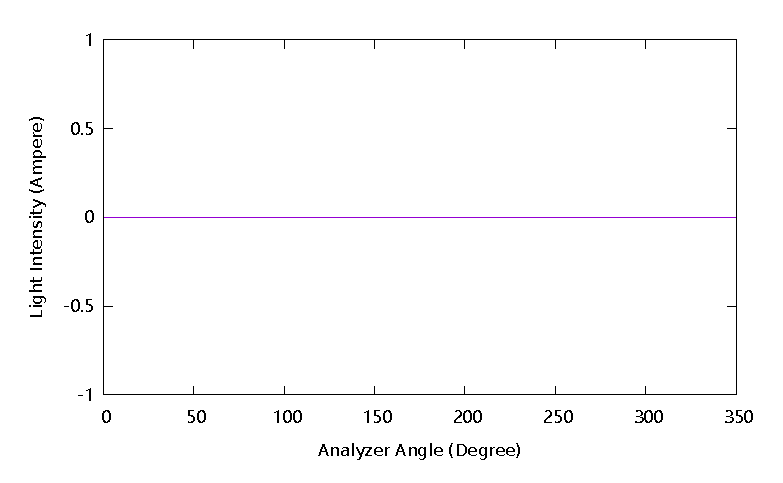
\includegraphics[width=\linewidth]{../output/analyzer-angle-light-intensity-9.gnuplot}
    \end{figure}
    \newpage
    \begin{table}[H]
        \centering
        \begin{tabular}{|c|c|c|c|c|c|c|c|c|c|}
            \hline
            检偏镜角度(${}^{\circ}$)  & 0    & 10   & 20   & 30   & 40   & 50   & 60   & 70   & 80   \\\hline
            光强($10^{-7} \si{A}$) & 0.00 & 0.00 & 0.00 & 0.00 & 0.00 & 0.00 & 0.00 & 0.00 & 0.00 \\\hline
            检偏镜角度(${}^{\circ}$)  & 90   & 100  & 110  & 120  & 130  & 140  & 150  & 160  & 170  \\\hline
            光强($10^{-7} \si{A}$) & 0.00 & 0.00 & 0.00 & 0.00 & 0.00 & 0.00 & 0.00 & 0.00 & 0.00 \\\hline
            检偏镜角度(${}^{\circ}$)  & 180  & 190  & 200  & 210  & 220  & 230  & 240  & 250  & 260  \\\hline
            光强($10^{-7} \si{A}$) & 0.00 & 0.00 & 0.00 & 0.00 & 0.00 & 0.00 & 0.00 & 0.00 & 0.00 \\\hline
            检偏镜角度(${}^{\circ}$)  & 270  & 280  & 290  & 300  & 310  & 320  & 330  & 340  & 350  \\\hline
            光强($10^{-7} \si{A}$) & 0.00 & 0.00 & 0.00 & 0.00 & 0.00 & 0.00 & 0.00 & 0.00 & 0.00 \\\hline
        \end{tabular}
        \caption{检偏器角度与光强关系,特定励磁电流$I=0.00 \si{A}$}
    \end{table}

    \begin{figure}[H]
        \centering
        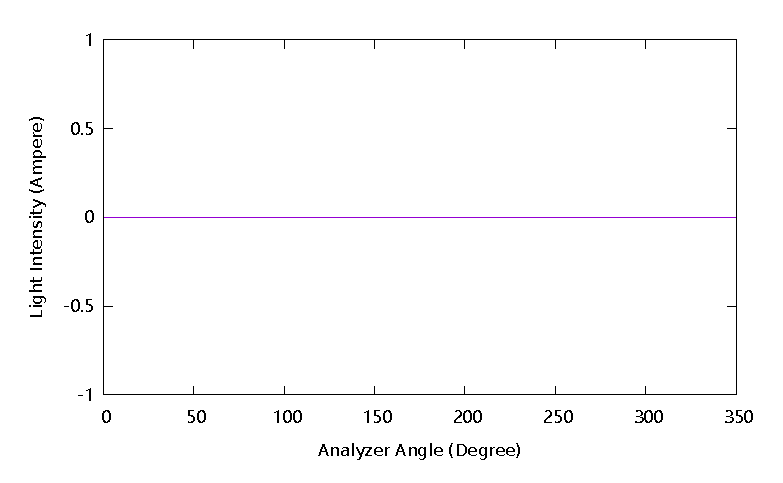
\includegraphics[width=\linewidth]{../output/analyzer-angle-light-intensity-10.gnuplot}
    \end{figure}
    \newpage
    \begin{table}[H]
        \centering
        \begin{tabular}{|c|c|c|c|c|c|c|c|c|c|}
            \hline
            检偏镜角度(${}^{\circ}$)  & 0    & 10   & 20   & 30   & 40   & 50   & 60   & 70   & 80   \\\hline
            光强($10^{-7} \si{A}$) & 0.00 & 0.00 & 0.00 & 0.00 & 0.00 & 0.00 & 0.00 & 0.00 & 0.00 \\\hline
            检偏镜角度(${}^{\circ}$)  & 90   & 100  & 110  & 120  & 130  & 140  & 150  & 160  & 170  \\\hline
            光强($10^{-7} \si{A}$) & 0.00 & 0.00 & 0.00 & 0.00 & 0.00 & 0.00 & 0.00 & 0.00 & 0.00 \\\hline
            检偏镜角度(${}^{\circ}$)  & 180  & 190  & 200  & 210  & 220  & 230  & 240  & 250  & 260  \\\hline
            光强($10^{-7} \si{A}$) & 0.00 & 0.00 & 0.00 & 0.00 & 0.00 & 0.00 & 0.00 & 0.00 & 0.00 \\\hline
            检偏镜角度(${}^{\circ}$)  & 270  & 280  & 290  & 300  & 310  & 320  & 330  & 340  & 350  \\\hline
            光强($10^{-7} \si{A}$) & 0.00 & 0.00 & 0.00 & 0.00 & 0.00 & 0.00 & 0.00 & 0.00 & 0.00 \\\hline
        \end{tabular}
        \caption{检偏器角度与光强关系,特定励磁电流$I=0.00 \si{A}$}
    \end{table}

    \begin{figure}[H]
        \centering
        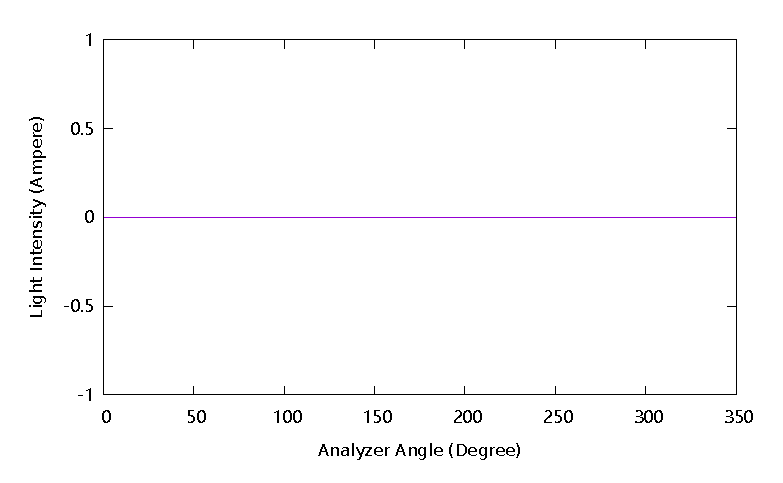
\includegraphics[width=\linewidth]{../output/analyzer-angle-light-intensity-11.gnuplot}
    \end{figure}
    \newpage
    \begin{table}[H]
        \centering
        \begin{tabular}{|c|c|c|c|c|c|c|c|c|c|}
            \hline
            检偏镜角度(${}^{\circ}$)  & 0    & 10   & 20   & 30   & 40   & 50   & 60   & 70   & 80   \\\hline
            光强($10^{-7} \si{A}$) & 0.00 & 0.00 & 0.00 & 0.00 & 0.00 & 0.00 & 0.00 & 0.00 & 0.00 \\\hline
            检偏镜角度(${}^{\circ}$)  & 90   & 100  & 110  & 120  & 130  & 140  & 150  & 160  & 170  \\\hline
            光强($10^{-7} \si{A}$) & 0.00 & 0.00 & 0.00 & 0.00 & 0.00 & 0.00 & 0.00 & 0.00 & 0.00 \\\hline
            检偏镜角度(${}^{\circ}$)  & 180  & 190  & 200  & 210  & 220  & 230  & 240  & 250  & 260  \\\hline
            光强($10^{-7} \si{A}$) & 0.00 & 0.00 & 0.00 & 0.00 & 0.00 & 0.00 & 0.00 & 0.00 & 0.00 \\\hline
            检偏镜角度(${}^{\circ}$)  & 270  & 280  & 290  & 300  & 310  & 320  & 330  & 340  & 350  \\\hline
            光强($10^{-7} \si{A}$) & 0.00 & 0.00 & 0.00 & 0.00 & 0.00 & 0.00 & 0.00 & 0.00 & 0.00 \\\hline
        \end{tabular}
        \caption{检偏器角度与光强关系,特定励磁电流$I=0.00 \si{A}$}
    \end{table}

    \begin{figure}[H]
        \centering
        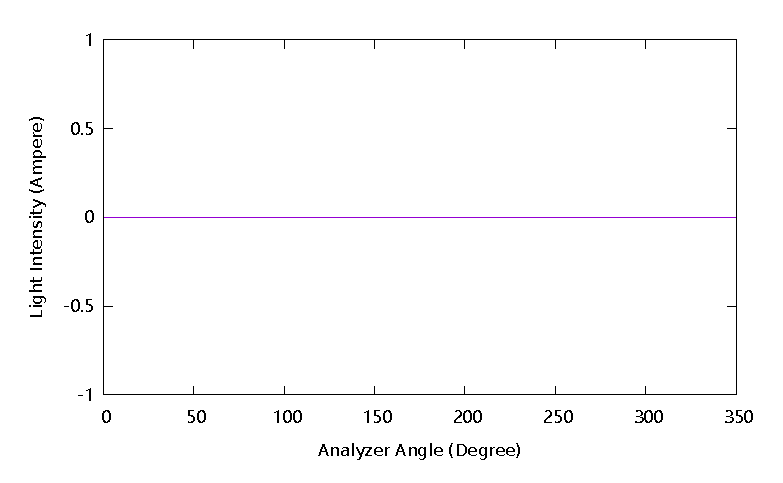
\includegraphics[width=\linewidth]{../output/analyzer-angle-light-intensity-12.gnuplot}
    \end{figure}
    \newpage
    \begin{table}[H]
        \centering
        \begin{tabular}{|c|c|c|c|c|c|c|c|c|c|}
            \hline
            检偏镜角度(${}^{\circ}$)  & 0    & 10   & 20   & 30   & 40   & 50   & 60   & 70   & 80   \\\hline
            光强($10^{-7} \si{A}$) & 0.00 & 0.00 & 0.00 & 0.00 & 0.00 & 0.00 & 0.00 & 0.00 & 0.00 \\\hline
            检偏镜角度(${}^{\circ}$)  & 90   & 100  & 110  & 120  & 130  & 140  & 150  & 160  & 170  \\\hline
            光强($10^{-7} \si{A}$) & 0.00 & 0.00 & 0.00 & 0.00 & 0.00 & 0.00 & 0.00 & 0.00 & 0.00 \\\hline
            检偏镜角度(${}^{\circ}$)  & 180  & 190  & 200  & 210  & 220  & 230  & 240  & 250  & 260  \\\hline
            光强($10^{-7} \si{A}$) & 0.00 & 0.00 & 0.00 & 0.00 & 0.00 & 0.00 & 0.00 & 0.00 & 0.00 \\\hline
            检偏镜角度(${}^{\circ}$)  & 270  & 280  & 290  & 300  & 310  & 320  & 330  & 340  & 350  \\\hline
            光强($10^{-7} \si{A}$) & 0.00 & 0.00 & 0.00 & 0.00 & 0.00 & 0.00 & 0.00 & 0.00 & 0.00 \\\hline
        \end{tabular}
        \caption{检偏器角度与光强关系,特定励磁电流$I=0.00 \si{A}$}
    \end{table}

    \begin{figure}[H]
        \centering
        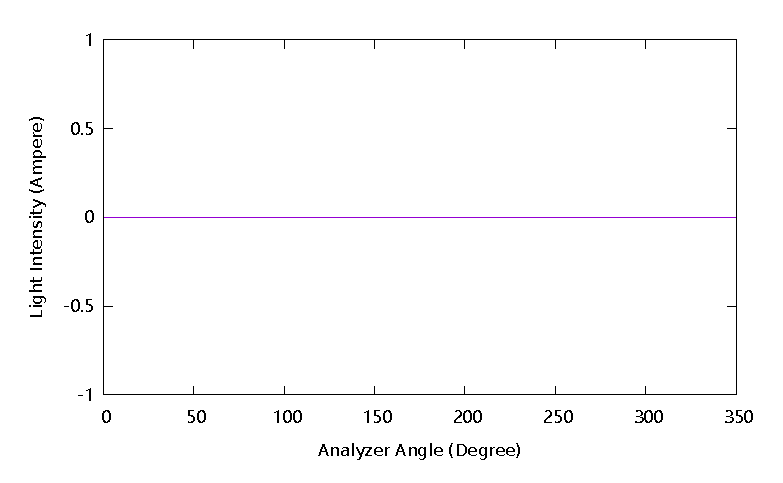
\includegraphics[width=\linewidth]{../output/analyzer-angle-light-intensity-13.gnuplot}
    \end{figure}
    \newpage
    \begin{table}[H]
        \centering
        \begin{tabular}{|c|c|c|c|c|c|c|c|c|c|}
            \hline
            检偏镜角度(${}^{\circ}$)  & 0    & 10   & 20   & 30   & 40   & 50   & 60   & 70   & 80   \\\hline
            光强($10^{-7} \si{A}$) & 0.00 & 0.00 & 0.00 & 0.00 & 0.00 & 0.00 & 0.00 & 0.00 & 0.00 \\\hline
            检偏镜角度(${}^{\circ}$)  & 90   & 100  & 110  & 120  & 130  & 140  & 150  & 160  & 170  \\\hline
            光强($10^{-7} \si{A}$) & 0.00 & 0.00 & 0.00 & 0.00 & 0.00 & 0.00 & 0.00 & 0.00 & 0.00 \\\hline
            检偏镜角度(${}^{\circ}$)  & 180  & 190  & 200  & 210  & 220  & 230  & 240  & 250  & 260  \\\hline
            光强($10^{-7} \si{A}$) & 0.00 & 0.00 & 0.00 & 0.00 & 0.00 & 0.00 & 0.00 & 0.00 & 0.00 \\\hline
            检偏镜角度(${}^{\circ}$)  & 270  & 280  & 290  & 300  & 310  & 320  & 330  & 340  & 350  \\\hline
            光强($10^{-7} \si{A}$) & 0.00 & 0.00 & 0.00 & 0.00 & 0.00 & 0.00 & 0.00 & 0.00 & 0.00 \\\hline
        \end{tabular}
        \caption{检偏器角度与光强关系,特定励磁电流$I=0.00 \si{A}$}
    \end{table}

    \begin{figure}[H]
        \centering
        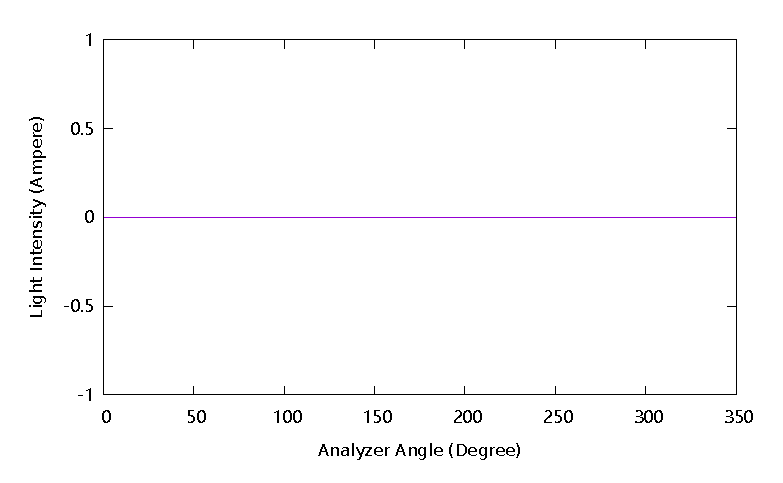
\includegraphics[width=\linewidth]{../output/analyzer-angle-light-intensity-14.gnuplot}
    \end{figure}
    \newpage
    \begin{table}[H]
        \centering
        \begin{tabular}{|c|c|c|c|c|c|c|c|c|c|}
            \hline
            检偏镜角度(${}^{\circ}$)  & 0    & 10   & 20   & 30   & 40   & 50   & 60   & 70   & 80   \\\hline
            光强($10^{-7} \si{A}$) & 0.00 & 0.00 & 0.00 & 0.00 & 0.00 & 0.00 & 0.00 & 0.00 & 0.00 \\\hline
            检偏镜角度(${}^{\circ}$)  & 90   & 100  & 110  & 120  & 130  & 140  & 150  & 160  & 170  \\\hline
            光强($10^{-7} \si{A}$) & 0.00 & 0.00 & 0.00 & 0.00 & 0.00 & 0.00 & 0.00 & 0.00 & 0.00 \\\hline
            检偏镜角度(${}^{\circ}$)  & 180  & 190  & 200  & 210  & 220  & 230  & 240  & 250  & 260  \\\hline
            光强($10^{-7} \si{A}$) & 0.00 & 0.00 & 0.00 & 0.00 & 0.00 & 0.00 & 0.00 & 0.00 & 0.00 \\\hline
            检偏镜角度(${}^{\circ}$)  & 270  & 280  & 290  & 300  & 310  & 320  & 330  & 340  & 350  \\\hline
            光强($10^{-7} \si{A}$) & 0.00 & 0.00 & 0.00 & 0.00 & 0.00 & 0.00 & 0.00 & 0.00 & 0.00 \\\hline
        \end{tabular}
        \caption{检偏器角度与光强关系,特定励磁电流$I=0.00 \si{A}$}
    \end{table}

    \begin{figure}[H]
        \centering
        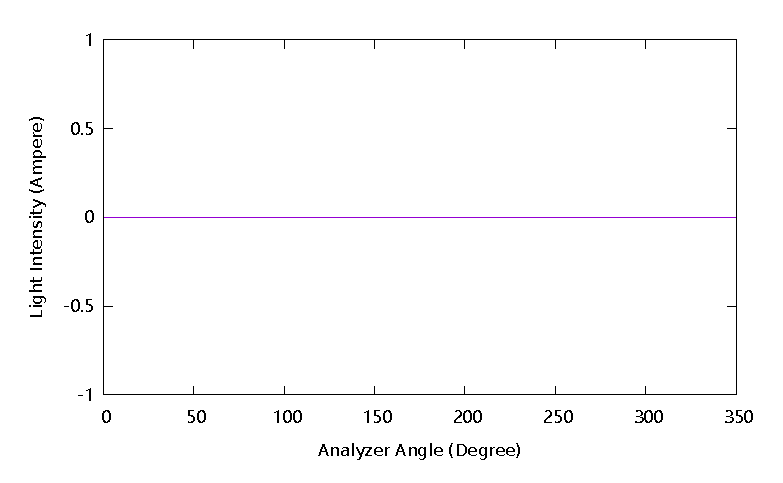
\includegraphics[width=\linewidth]{../output/analyzer-angle-light-intensity-15.gnuplot}
    \end{figure}
    \newpage
    \begin{table}[H]
        \centering
        \begin{tabular}{|c|c|c|c|c|c|c|c|c|c|}
            \hline
            检偏镜角度(${}^{\circ}$)  & 0    & 10   & 20   & 30   & 40   & 50   & 60   & 70   & 80   \\\hline
            光强($10^{-7} \si{A}$) & 0.00 & 0.00 & 0.00 & 0.00 & 0.00 & 0.00 & 0.00 & 0.00 & 0.00 \\\hline
            检偏镜角度(${}^{\circ}$)  & 90   & 100  & 110  & 120  & 130  & 140  & 150  & 160  & 170  \\\hline
            光强($10^{-7} \si{A}$) & 0.00 & 0.00 & 0.00 & 0.00 & 0.00 & 0.00 & 0.00 & 0.00 & 0.00 \\\hline
            检偏镜角度(${}^{\circ}$)  & 180  & 190  & 200  & 210  & 220  & 230  & 240  & 250  & 260  \\\hline
            光强($10^{-7} \si{A}$) & 0.00 & 0.00 & 0.00 & 0.00 & 0.00 & 0.00 & 0.00 & 0.00 & 0.00 \\\hline
            检偏镜角度(${}^{\circ}$)  & 270  & 280  & 290  & 300  & 310  & 320  & 330  & 340  & 350  \\\hline
            光强($10^{-7} \si{A}$) & 0.00 & 0.00 & 0.00 & 0.00 & 0.00 & 0.00 & 0.00 & 0.00 & 0.00 \\\hline
        \end{tabular}
        \caption{检偏器角度与光强关系,特定励磁电流$I=0.00 \si{A}$}
    \end{table}

    \begin{figure}[H]
        \centering
        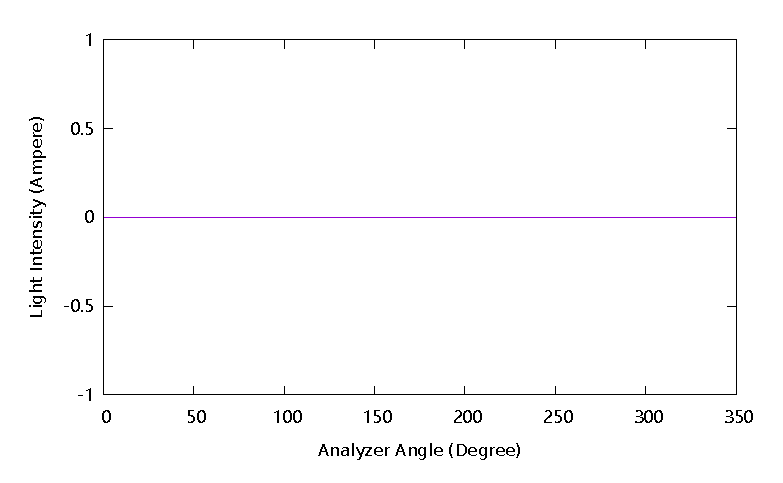
\includegraphics[width=\linewidth]{../output/analyzer-angle-light-intensity-16.gnuplot}
    \end{figure}
    \newpage
    \begin{table}[H]
        \centering
        \begin{tabular}{|c|c|c|c|c|c|c|c|c|c|}
            \hline
            $I/(\si{mA})$ & 0.00 & 0.00 & 0.00 & 0.00 & 0.00 & 0.00 & 0.00 \\\hline
            $U / \si{V}$  & 1.00 & 1.00 & 1.00 & 1.00 & 1.00 & 1.00 & 1.00 \\\hline
            $P / \si{mW}$ & 2.00 & 2.00 & 2.00 & 2.00 & 2.00 & 2.00 & 2.00 \\\hline
        \end{tabular}
        \caption{LED,温度$T=25.00$}
    \end{table}
    \newpage
    \begin{table}[H]
        \centering
        \begin{tabular}{|c|c|c|c|c|c|c|c|c|c|}
            \hline
            $I/(\si{mA})$ & 0.00 & 0.00 & 0.00 & 0.00 & 0.00 & 0.00 & 0.00 \\\hline
            $U / \si{V}$  & 0.00 & 0.00 & 0.00 & 0.00 & 0.00 & 0.00 & 0.00 \\\hline
            $P / \si{mW}$ & 0.00 & 0.00 & 0.00 & 0.00 & 0.00 & 0.00 & 0.00 \\\hline
        \end{tabular}
        \caption{LED,温度$T=0.00$}
    \end{table}
    \newpage
    \begin{table}[H]
        \centering
        \begin{tabular}{|c|c|c|c|c|c|c|c|c|c|}
            \hline
            $I/(\si{mA})$ & 0.00 & 0.00 & 0.00 & 0.00 & 0.00 & 0.00 & 0.00 \\\hline
            $U / \si{V}$  & 0.00 & 0.00 & 0.00 & 0.00 & 0.00 & 0.00 & 0.00 \\\hline
            $P / \si{mW}$ & 0.00 & 0.00 & 0.00 & 0.00 & 0.00 & 0.00 & 0.00 \\\hline
        \end{tabular}
        \caption{LED,温度$T=0.00$}
    \end{table}
    \newpage
    \begin{table}[H]
        \centering
        \begin{tabular}{|c|c|c|c|c|c|c|c|c|c|}
            \hline
            $I/(\si{mA})$ & 0.00 & 0.00 & 0.00 & 0.00 & 0.00 & 0.00 & 0.00 \\\hline
            $U / \si{V}$  & 0.00 & 0.00 & 0.00 & 0.00 & 0.00 & 0.00 & 0.00 \\\hline
            $P / \si{mW}$ & 0.00 & 0.00 & 0.00 & 0.00 & 0.00 & 0.00 & 0.00 \\\hline
        \end{tabular}
        \caption{LED,温度$T=0.00$}
    \end{table}
    \newpage
    \begin{table}[H]
        \centering
        \begin{tabular}{|c|c|c|c|c|c|c|c|c|c|}
            \hline
            $I/(\si{mA})$ & 0.00 & 0.00 & 0.00 & 0.00 & 0.00 & 0.00 & 0.00 \\\hline
            $U / \si{V}$  & 0.00 & 0.00 & 0.00 & 0.00 & 0.00 & 0.00 & 0.00 \\\hline
            $P / \si{mW}$ & 0.00 & 0.00 & 0.00 & 0.00 & 0.00 & 0.00 & 0.00 \\\hline
        \end{tabular}
        \caption{LED,温度$T=0.00$}
    \end{table}
    \newpage
    \begin{table}[H]
        \centering
        \begin{tabular}{|c|c|c|c|c|c|c|c|c|c|}
            \hline
            $I/(\si{mA})$ & 0.00 & 0.00 & 0.00 & 0.00 & 0.00 & 0.00 & 0.00 \\\hline
            $U / \si{V}$  & 0.00 & 0.00 & 0.00 & 0.00 & 0.00 & 0.00 & 0.00 \\\hline
            $P / \si{mW}$ & 0.00 & 0.00 & 0.00 & 0.00 & 0.00 & 0.00 & 0.00 \\\hline
        \end{tabular}
        \caption{LED,温度$T=0.00$}
    \end{table}
    \newpage


    \section{参考文献}
    \begin{itemize}[leftmargin=0pt]
        \item[] 综合物理实验讲义
    \end{itemize}
\end{document}